%old \documentclass[a4paper,12pt,headsepline,smallheadings]{scrreprt} %scrartcl, scrbook
\documentclass[a4paper,
                          headsepline,
                          listof=totoc,
                          toc=listof,
                          headings=small]{scrreprt} %scrartcl, scrapbook

\usepackage{amsmath,amssymb,amsfonts} % Typical maths resource packages
\usepackage{graphics}                 % Packages to allow inclusion of graphics
\usepackage{color}                    % For creating coloured text and background
\usepackage[english]{babel}
\usepackage[applemac]{inputenc}
\usepackage{wrapfig}

% line spacing
%\renewcommand{\baselinestretch}{1.3}
\usepackage{setspace}
\onehalfspacing

%\usepackage{geometry} % page margins
%\geometry{a4paper, left=2.5cm, right=2.5cm, top=2.5cm, bottom=2.5cm}

% index pages
\usepackage{makeidx}
\makeindex

% graphicx figures
\usepackage{graphicx}
\DeclareGraphicsExtensions{.pdf,.jpg,.gif}

% mini table of contents in each chapter
%\usepackage[undotted]{minitoc}
%\mtcselectlanguage{english}
%\nomtcpagenumbers
%\nomtcrule

%\setuptoc{toc}{totoc}

%\usepackage{fancyhdr}
%\pagestyle{fancy}

% fancy chapter style
\usepackage[Lenny]{fncychap/fncychap}
\ChTitleVar{\bfseries\Large\rmfamily}
\ChNameVar{\bfseries\Large\sffamily}

% For creating hyperlinks in cross references
\usepackage[pdftex,bookmarks,colorlinks]{hyperref}
\hypersetup{colorlinks,citecolor=black,filecolor=black,linkcolor=black,urlcolor=black,plainpages=false}

%---------------------------------------------------------------------------------------------

%footnote without number
%\renewcommand{\thefootnote}{\fnsymbol{footnote}}
%\def\blfootnote{\xdef\@thefnmark{}\@footnotetext}
\long\def\symbolfootnote[#1]#2{\begingroup%
\def\thefootnote{\fnsymbol{footnote}}\footnote[#1]{#2}\endgroup}

% additional
\newcommand{\areps}{\textit{Ann.\ Rev.\ Earth planet\ Sci.,} }
\newcommand{\bssa}{\textit{Bull.\ seism.\ Soc.\ Am.,} }
\newcommand{\eos}{\textit{EOS, Trans.\ Am.\ geophys.\ Un.,} }
\newcommand{\eps}{\textit{Earth~Planets~Space},}
\newcommand{\epsl}{\textit{Earth~planet.\ Sci.\ Lett.,} }
\newcommand{\gca}{\textit{Geochim.\ Cosmochim.\ Acta,} }
\newcommand{\geo}{\textit{Geology,} }
\newcommand{\geop}{\textit{Geophysics,} }
\newcommand{\gji}{\textit{Geophys.\ J.\ Int.,} }
\newcommand{\gjras}{\textit{Geophys.\ J.\ R.\ astr.\ Soc.,} }
\newcommand{\grl}{\textit{Geophys.\ Res.\ Lett.,} }
\newcommand{\gsab}{\textit{Geol.\ Soc.\ Am.\ Bull.},}
\newcommand{\gs}{\textit{Geophys.\ Surv.,} }
\newcommand{\jgr}{\textit{J.\ geophys.\ Res.,} }
\newcommand{\jpo}{\textit{J.\ Phys.\ Oceanogr.,} }
\newcommand{\jseis}{\textit{J.~Seism.,} }
\newcommand{\mnras}{\textit{Mon.\ Not.\ R.\ astr.\ Soc.,} }
\newcommand{\pag}{\textit{Pure appl.\ Geophys.},}
\newcommand{\pepi}{\textit{Phys.\ Earth planet.\ Inter.,} }
\newcommand{\rg}{\textit{Rev.\ Geophys.,} }
\newcommand{\tecto}{\textit{Tectonophysics,} }
\newcommand{\sjna}{\textit{SIAM~J.~Num.~Anal.,} }
\newcommand{\sjsc}{\textit{SIAM~J.~Sci.~Comp.,} }
\newcommand{\mi}{\textit{Math.~Intelligencer,} }


%-------------------------------------------------------------------------------------------------------------
%% DOCUMENT
%-------------------------------------------------------------------------------------------------------------
\begin{document}

%\frontmatter
%\mainmatter

%-------------------------------------------------------------------------------------------------------------
%%TITLE
%-------------------------------------------------------------------------------------------------------------
\thispagestyle{empty}
%\vspace{-4.0cm}

\noindent
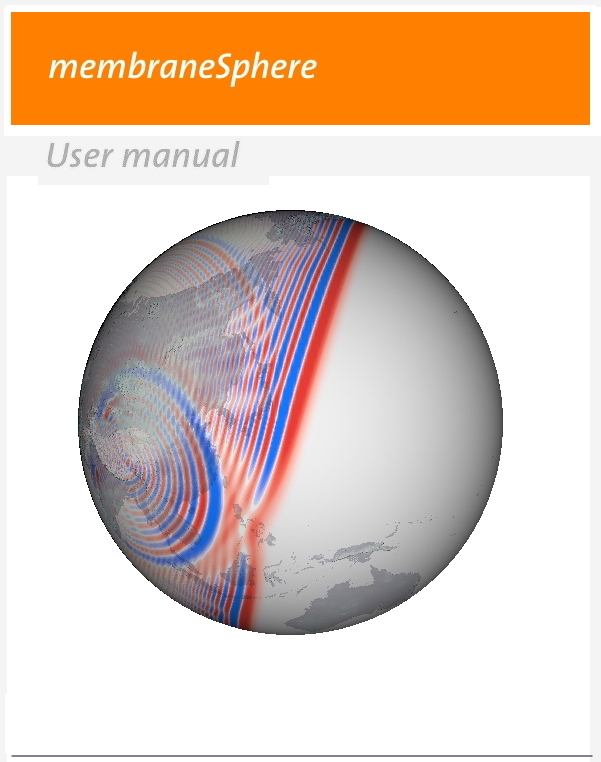
\includegraphics[width=1.0\textwidth]{figures/title_plain5.jpg}

\newpage
\thispagestyle{empty}

\begin{samepage}

\noindent
\vspace{12cm}\\

%---------------------------------------------------------------------------------------------
% TITLE & AUTHOR
%
\title{membraneSphere\\User Manual}

% version
\author{Version 1.2}

% date of last edit
\date{{\small  \copyright   \today }}

\maketitle


\end{samepage}

%-------------------------------------------------------------------------------------------------------------
% 	Table of contents
%-------------------------------------------------------------------------------------------------------------
%\dominitoc[n]
%	\mtcaddchapter
%\tableofcontents
%	%\mtcaddchapter[Contents]
%	\mtcaddchapter
%	%\addcontentsline{toc}{chapter}{Inhaltsverzeichnis}

\renewcommand{\contentsname}{Table of Contents}
\tableofcontents

%---------------------------------------------------------------------------------------------
\chapter{Introduction}
%---------------------------------------------------------------------------------------------
\texttt{membraneSphere} is a software package to simulate waves on a spherical
membrane. It implements the membrane wave method introduced by {Tanimoto (1990)}.
Membrane waves are an analogue for seismic surface waves. The zero-thickness
sphere is discretized by a geodesic grid ({Tape}, 2003). Wave propagation on
this sphere is solved by a finite-difference scheme for such
hexagonal grids (Tape, 2003; {Heikes \& Randall}, 1995a).

If you intent to use \texttt{membraneSphere}, please reference the
following articles:
\\
\\
Tanimoto, T., 1990.
\textit{Modelling curved surface wave paths: membrane surface wave synthetics},
\gji \textbf{102}, 89--100.
\\
\\
Tape, C. H., 2003.
\textit{Waves on a Spherical Membrane},
M.Sc. thesis, University of Oxford, U.K.
\\
\\
Peter, D., C. Tape, L. Boschi and J. H. Woodhouse, 2007.
\textit{Surface wave tomography: global membrane waves and adjoint methods},
\textit{\gji}, \textit{171}: p. 1098-1117.\\


%---------------------------------------------------------------------------------------------
\chapter{Getting started}
%---------------------------------------------------------------------------------------------
The codes are written in Fortan90. You should use the appropriate compiler flags
in the \texttt{Makefile} by setting \textsf{F90}, \textsf{FFLAGS} and \textsf{LDFLAGS}
to fit your installation.


In \texttt{src/include/commonModules.f90} you have to choose the precision (single
precision is default), the source parameters explained in {Tape} (2003)
and the filtering parameters prior to compilation. To create the binaries, use
the command \textsf{make}.


In \texttt{Parameter\_Input} choose the physical model (grid refinement level,
simulation times and wave type) and set the source/receiver geometry. You can also place
a single scatterer and/or use a heterogeneous background phase-velocity model. These
parameters are read in when the program starts. They can be changed without
the need of recompilation of the programs.




%---------------------------------------------------------------------------------------------
\chapter{Using a mesh}
%---------------------------------------------------------------------------------------------
%\section{Employing meshes}
There are data files containing the coordinations of grid points and cells for a geodesic grid
({Tape}, 2003) located in the directory \texttt{data/griddata/}. To choose a certain refinement level
of the grid, you set the parameter \textbf{LEVEL} in the file \texttt{Parameter\_Input}
to a value between $0$ and $6$.

\vspace{2cm}
\begin{center}
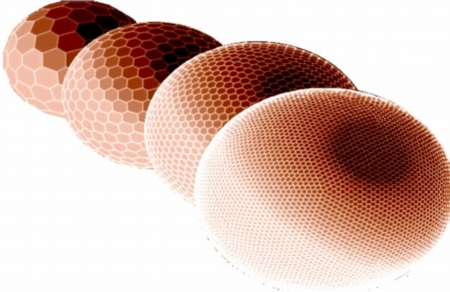
\includegraphics[width=0.8\textwidth]{figures/spheres.jpg}
\end{center}



%---------------------------------------------------------------------------------------------
\chapter{Performing a simulation}
%---------------------------------------------------------------------------------------------
The main executable is \texttt{propagation}.
It calculates a simulation of membrane waves propagating over a sphere.
It reads the main input file \texttt{Parameter\_Input}:
\\
\begin{itemize}
\item{\textbf{LEVEL}}
sets the subfolding level of the hexagonal grid. It can be an integer value
between $0$ (coarsest) to $6$ (finest grid).

\item \textbf{FIRSTTIME}
determines the starting time (in seconds) of the simulation. In order to properly account for the analytical source (Tape, 2003), the default is set to $-1000.0$ s.

\item \textbf{LASTTIME}
determines the end time (in seconds) of the simulation.

\item \textbf{CPHASE}
sets the phase-velocity of the seismic wave which will be simulated. This value
will determine the background phase-velocity in (km/s) set on the membrane.

It is given in as a combination format, first of the type, either Rayleigh (R) or Love (L) wave, and the wave period (available wave periods in seconds are: 35, 37, 40, 45, 50, 60, 75, 100, 150, 200, 250 or 300), e.g. if one wants Love waves at 150 s period it is set to \textit{L150}.

\item \textbf{SOURCE}
sets latitude and longitude (in degrees) for the source location.

\item \textbf{RECEIVER}
sets latitude and longitude (in degrees) for the receiver location.
The simulation will output the wave displacements calculated for this location.


\vspace{2cm}
%\begin{center}
\hspace{-1cm}
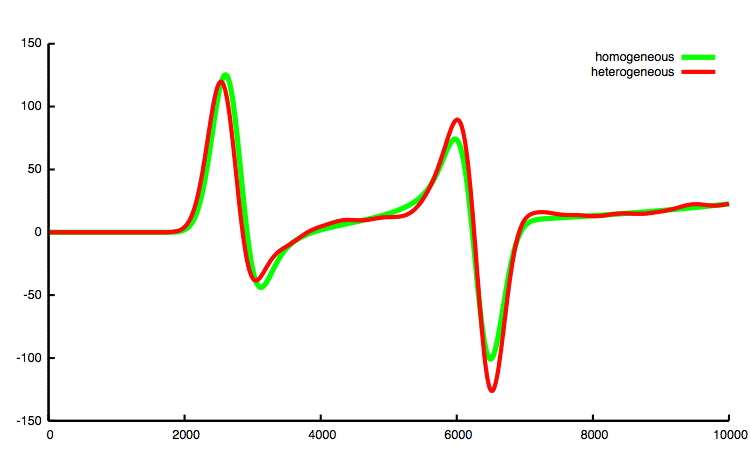
\includegraphics[width=1.0\textwidth]{figures/homheterogeneousL35.jpg}
%\end{center}




\item \textbf{MANYRECEIVERS}
can be either \textit{true} or \textit{false} depending if one wants to run a simulation
with a geometrical optimization where many receivers were placed on the same latitude in order to perform a direct sensitivity kernel calculation (see Peter et al. 2007).

\item \textbf{MANYNUMOFRECEIVERS}
sets the number of many receivers to be used for the geometrical optimization from above. It is only required when MANYRECEIVERS is set to be true.

\item \textbf{MANYKERNELS}
can be either \textit{true} or \textit{false}. It performs a loop over the range of given epicentral distances to calculate sensitivity kernels.

\item \textbf{KRNEPI}
sets the range of epicentral distances, i.e. the minimum and maximum distance (in degrees) for the loop over many kernels. Only if MANYKERNELS is set to true it is required.

\item \textbf{IMPORTKERNELSRECEIVERS}
can be either \textit{true} or \textit{false}. It reads the different receiver locations from
a file. The file name must be called "tmpReceiverStations***.dat"

\item \textbf{DELTA}
can be either \textit{true} or \textit{false}. It is used if one want to place a single scatterer
on the membrane.

\item \textbf{DRADIUS}
determines the radius size of the single scatterer (in km). If one wants only a single cell
to be perturbed, it is set to a value smaller than the grid spacing, e.g. 0.1.

\item \textbf{DTYPE}
can be either \textit{plateau} or \textit{gaussian}. The perturbation is multiplied by
a normalization function. This function is either given by
a function set to 1 where the grid point location is inside the radius of the scatterer
or 0 everywhere else (\textit{plateau}). The other normalization is given by a gaussian function with a smooth transition from 0 for locations further away
than the radius to 1 at the center of the scatterer location (\textit{gaussian}).

\item \textbf{DPERTURBATION}
sets the perturbation size (in km/s) of the phase velocity at the scatterer location.

\item \textbf{DLOCATION}
sets latitude and longitude (in degrees) of the scatterer location.


\item \textbf{MOVEDELTA}
can be either \textit{true} or \textit{false}. In case one wants to calculate a sensitivity kernel
in a direct way (see Peter et al. 2007). It loops over many simulations
with each time a slightly different scatterer location.

\item \textbf{DLATSTART}
determines the starting latitude (in degrees) of the scatterer location. It is only
considered in case MOVEDELTA is set.

\item \textbf{DLATEND}
determines the latitude (in degrees) of the scatterer for the last simulation. It is only considered in case MOVEDELTA is set.

\item \textbf{DLONEND}
determines the longitude (in degrees) of the scatterer for the last simulation. It is
only considered in case MOVEDELTA is set.

\item \textbf{DINCREMENT}
gives the incremental step size (in degrees) to take from one simulation
to the next one. The scatterer location is moved by this amount, first for a
loop over latitudes and then a loop over longitudes. It is only considered in case MOVEDELTA is set.

\item \textbf{SECONDDELTA}
can be either \textit{true} or \textit{false}. If set, a second scatterer is placed (details
can be set in the file commonModules.f90) on the membrane
together with the delta scatterer set above. It is only considered in case DELTA is set.

\item \textbf{HETEROGENEOUS}
can be either \textit{true} or \textit{false}. If set to true, a heterogeneous phase-velocity distribution must be specified which will be set as background map on the membrane.
If not set, the membrane will have a uniform, constant phase-velocity over the whole sphere, with a value set to the wave type and period specified by parameter CPHASE.

\item \textbf{BLKFILE}
specifies the file name of a heterogeneous phase-velocity distribution.
You have two possibilities:

(a) choose a block file e.g. "L150.crust.2degree.3.pcn.blk", then BLK/INV\_PIXELSIZE must be set to the size of the blocks (e.g. 3 for a 3x3 degree pixel size).

(b) choose a general spherical harmonics file e.g. "L150.crust.2degree.gsh" (derived by CRUST2.0 for Love waves at 150 s period), then BLK/INV\_PIXELSIZE must be set to the degree of expansion you want (e.g. 12 for expansion up to degree 12).

(Make sure that the path to the file is given in the correct form: it might include to have a full path, e.g.\\
"data/phasedata/L150.crust.2degree.3.pcn.blk".)

It is only considered if HETERGENEOUS is set.

\item \textbf{BLK/INV\_PIXELSIZE}
see above. It is only considered if HETERGENEOUS is set.

\item \textbf{BLKVELOCITYREFERENCE}
set the type of surface wave and period for which the heterogeneous distributions
are given. The distributions are given as percentage of perturbations to this reference.

\item \textbf{INV\_DATA}
specifies the file name with a list of source-station setups
like e.g. "wei\_sum.02.L0150.1.txt",
used for the executable \texttt{heterogeneousPhaseshift} (otherwise not required)
in order to calculate the phase-anomalies for each source-station pair.

(Make sure that the path to the file is given in the correct form: it might include to have a full path, e.g.\\
"data/phasedata/wei\_sum.02.L0150.1.txt".)


It requires a heterogeneous background phase-velocity map
(see HETEROGENEOUS).


\item \textbf{INV\_OUTPUT}
not required.

\item \textbf{INV\_VOXELSIZE}
not required.

\item \textbf{DATADIRECTORY}
sets the name of the direction where output files are written to.

\item \textbf{ADJOINTKERNEL}
is optional and only considered for adjoint kernel calculations. It sets the file name
for the output kernel values.

\item \textbf{VERBOSE}
can be either \textit{true} or \textit{false} depending if one wants the console output to be verbose.

\item \textbf{SIMULATIONOUTPUT}
can be either \textit{true} or \textit{false}. If true, the simulation will write out the
complete forward wavefield at a regular time
interval (details can be specified in file commonModules.f90).

This output can be used to visualize the displacements as a movie.

\item \textbf{PARALLELSEISMO}
can be either \textit{true} or \textit{false}. If set to true, the code runs in parallel on using MPI
to communicate. The executable must be run either by mpirun or mpiexec.
\\
\\
(Additional detailed parameters can be set
in the file include/commonModules.f90 file.)

\end{itemize}


Main program output is the seismogram (format: time / displacement, with the
time given in seconds),
written in the data directory DATADIRECTORY specified in Parameter\_Input.
\\
\\
For checking purposes, it also outputs the used phase map
(format: longitude / latitude / phasespeed)
and the phase speed squared at the vertices
(format: verticeID / phasespeedsquared).

Visualization of the seismograms can be done with the GNUPLOT application.
The \texttt{scripts/} folder holds a bash-script for visualization of the
phase-map with GMT.

%---------------------------------------------------------------------------------------------
\chapter{Computing a sensitivity kernel}
%---------------------------------------------------------------------------------------------
\begin{flushright}
%\hspace{-1cm}
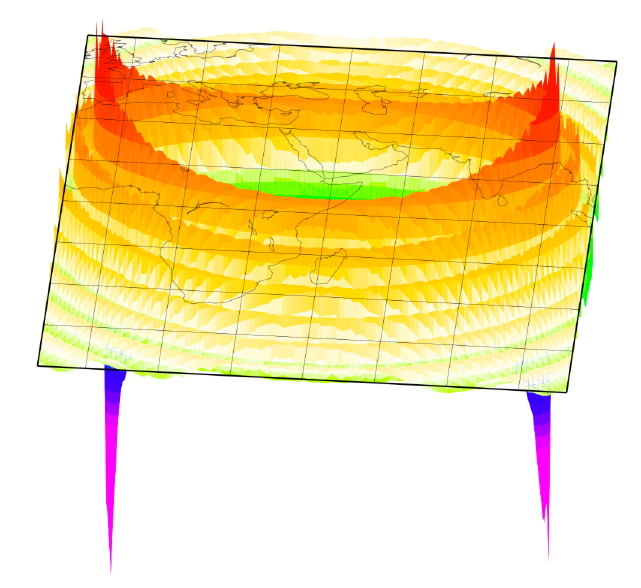
\includegraphics[width=0.5\textwidth]{figures/adjointkernel-L150-3D.jpg}
\end{flushright}

You can construct sensitivity kernels by membrane waves.
The executable \texttt{adjointMethod} performs a simulation, where no scatterer is present,
and calculates the adjoint source.
Then it makes a time-reversed simulation and computes the kernel values.
\\
\\
It reads the main input file \texttt{Parameter\_Input}. For details, look in the former
section. More specified parameters can be set
in the file \texttt{commonModules.f90} which is located in the \texttt{includes/} source directory.

\vspace{2cm}
\begin{center}
%\hspace{-1cm}
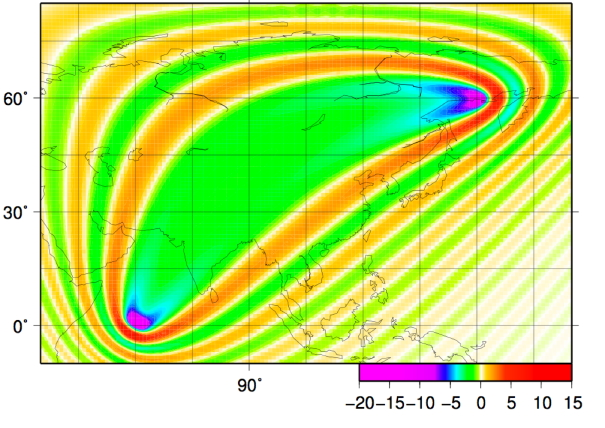
\includegraphics[width=1.0\textwidth]{figures/tibet-adjointHet40.jpg}
\end{center}

The kernel values are written to an output file in the data directory and with a name
specified in file \texttt{Parameter\_Input}. The output file format is: longitude / latitude / kernelvalue / vertexID.
Kernel values are evaluated at the vertices of the (triangular)
spherical membrane grid only.


To visualize the kernel, there are two bash-scripts in the \texttt{scripts/} folder
using GMT. These scripts \texttt{gmtplot\_2Dkernel.sh} (plot as 2D map) and
\texttt{gmtplot\_3Dkernel.sh} (plot in 3D perspective) interpolate the kernel file
and output cross-sections at different longitudes as well.




\appendix
%---------------------------------------------------------------------------------------------
\chapter{Utilities}
%---------------------------------------------------------------------------------------------

The source timelag.f90 calculates the phase shift/time shift of two seismograms.
This utility program calculates the time lag between two seismograms.

It reads only the input file Timelag\_Input. Other parameters (especially
the filter parameters) are taken from commonModules.f90.

The time shift result is written to the console.


%---------------------------------------------------------------------------------------------
\chapter{Post-processing scripts}
%---------------------------------------------------------------------------------------------
There are several scripts to visualize your results. They are located in the
directory \texttt{scripts/}.


\begin{itemize}
  \item
The \textit{gmtplot} scripts use the GMT
(Generic Mapping Tools) data processing and display software package Version 4.0.
They also make use of the color table files in the directory.

  \item
The \textit{gnuplot} scripts use the Gnuplot plotting utility Version 4.0.

  \item
The shell scripts employ the utilities Gawk Version 3.1 and Python Version 2.3.

\end{itemize}


%---------------------------------------------------------------------------------------------
\chapter{Copyright}
%---------------------------------------------------------------------------------------------
%\addcontentsline{toc}{chapter}{Copyright}

The software shall be used for scientific purposes only, excluding industrial or commercial purposes.

The software is furnished on an "as is" basis and the copyright holder in no way warrants
the software or any of its results and is in no way liable for any use made of the software.
The copyright holder disclaims all warranties, representations, and statements, express or implied, statutory or otherwise, including, without limitation, any implied warranties of
merchantability or fitness for a particular purpose.

In no event shall the copyright holder be liable for any actual, direct, indirect, special, consequential, or incidental damages, however caused, including, without limitation, any damages arising out of the use or operation of the software, loss of use of the software, or damage of any sort to the user.


%---------------------------------------------------------------------------------------------
\chapter{Notes and Acknowledgement}
%---------------------------------------------------------------------------------------------
%\addcontentsline{toc}{chapter}{Notes and Acknowledgement}

Note that subroutines from "Numerical Recipes: The Art of Scientific Computing"
by W. H. Press et al., Cambridge University Press, are used in
numericalRecipes*.f90. The user must acquire an official
Numerical Recipes license to run them.

The parallel computing is done using the implementation MPICH of the standard message passing
interface (MPI). It is freely available under \href{http://www-unix.mcs.anl.gov}{http://www-unix.mcs.anl.gov}.


% ------------------------------------------------------------------------
%  REFERENCE LIST
% ------------------------------------------------------------------------
%\backmatter

%\bibliographystyle{nature}
\begin{thebibliography}{Bibliography}
%	\mtcaddchapter[\bibname]
\addcontentsline{toc}{chapter}{\bibname}

\bibitem{15} Heikes, R. and D. A. Randall, 1995.
{Numerical integration of the shallow-water equations on a twisted icosahedral grid.1.
Basic design and results of tests}, \textit{Mon. Weather Rev.}, \textbf{123}, 1862--1880.

\bibitem{16} Heikes, R. and D. A. Randall, 1995.
{Numerical integration of the shallow-water equations on a twisted icosahedral grid.2.
A detailed description of the grid and an analysis of numerical accuracy},
\textit{Mon. Weather Rev.}, \textbf{123}, 1881--1887.

\bibitem{1} Peter, D., C. Tape, L. Boschi and J. H. Woodhouse, 2007. Surface wave tomography: global membrane waves and adjoint methods, \textit{\gji}, \textit{171}: p. 1098-1117.

\bibitem{36b} Tanimoto, T., 1990.
{Modelling curved surface wave paths: membrane surface wave synthetics}, \gji \textbf{102}, 89--100.

\bibitem{37b} Tape, C. H., 2003.
\textit{Waves on a Spherical Membrane}, M.Sc. thesis, University of Oxford, U.K.

\end{thebibliography}


%\newpage
%\phantomsection
% \addcontentsline{toc}{chapter}{\indexname}
%\printindex

\end{document}

